%%%%
\section{Poluição do Ar}

A poluição do ar resulta de uma complexa mistura de emissões naturais e 
antropogênicas, estima-se que ela seja responsável por 3,2 milhões de mortes 
por ano no mundo todo \citep{lim2013}. 

All in all, motor vehicle traffic is the most important
source of air pollution in cities, and according to Lamarque
et al. (2010), transportation is the predominant source of
anthropogenic black carbon (BC) in Latin America.
Johansson et al. (2007) also showed that road traffic emissions
are a major contributor to the number concentration of
ultrafine particles in urban environments, because the bulk
proportion of particles generated from gasoline and diesel
combustion are smaller than 60 nm and 100 nm, respectively
(Kittelson, 1998; Gouriou et al., 2004)

Diesel-powered
vehicles, which are usually a smaller fraction of the fleet,
make a proportionally large contribution to total number
concentrations (Kittelson et al., 2006). For example, Krecl et
al. (2015) showed that 73% of BC particles in Stockholm
come from diesel emissions, especially in the early hours at
weekends.

A inalação de material particulado $MP$ exerce um papel importante na 
exacerbação de doenças respiratórias, incluindo enfisema pulmonar e asma. 
Suas pequenas dimensões e massa, facilitam a penetração do $MP$ no sistema 
respiratório. 

A deposição no sistema respiratório humano ocorre em função do diâmetro da 
partícula.
As partículas grossas $MP_{2,5-10}$ ficam retidas no nariz (nasofaringe) e
as partículas mais finas $MP_{2,5}$ chegam nos alvéolos pulmonares e 
nos bronquíolos.
Nas áreas danificadas ocorre o comprometimento das trocas gasosas podendo, 
também, acarretar problemas cardiovasculares.
O próprio corpo consegue remover partículas através do macrófago alveolar 
e do sistema linfático \citep{arbex2012}.

%Os vírus são $MP_{2,5}$ e bactérias são $MP_{10}$ 
%o que significa que vírus tem maior penetração.

%%%%
\subsection{Material Particulado $MP$}

Material Particulado $MP$ ou Aerossóis Atmosféricos são partículas
sólidas ou líquidas em suspensão em um gás, as quais tem diâmetro 
aerodinâmico compreendido  entre $0,001-100\mu m$. 
A parte considerada inalável para humanos tem diâmetro menor que 10 $\mu m$
e se comporta praticamente como gás.
As partículas maiores que 10 $\mu m$ têm dificuldade em penetrar 
no sistema respiratório porque seu arraste pelo ar inalado não vence 
a força da gravidade \citep{seinfeld1998}.

O $MP$ pode ser classificado por tamanho, formação 
(primária ou secundária), pela forma de remoção da atmosfera, 
composição química ou forma geométrica da partículas \citep{seinfeld1998}.

A divisão por tamanho separa o $MP$ menor de $10 \mu m$ em quatro modas:
ultra-finas, núcleos de Aitken, acumulação e grossa. 

\begin{itemize}
  \item \textbf{ultra-finas:} formada por vapores de baixa votatilidade;
  \item \textbf{nucleação ou núcleos de Aitken:} 
        gerada a partir da condensação de vapores quentes ou durante o processo de 
        transformação de gás em partícula. Partículas formadas por 
        nucleação são removidas da atmosfera por aglomeração.   
  \item \textbf{moda acumulação:} 
         partículas na moda de acumulação são criadas 
         a partir de núcleos de condensação (núcleos de Aitken) através da 
         coagulação ou condensação de vapores. 
         Partículas formadas por acumulação
         são removidas da atmosfera por deposição seca ou úmida.
  \item \textbf{moda grossa ($MP_{2,5-10}$):} 
        são oriundas de processos mecânicos como fragmentação, 
        movimentação e manuseio. Partículas grossas são removidas da atmosfera 
        por sedimentação.
\end{itemize}

A figura proposta por \citep{finlayson1999} ilustra os processos de 
formação e remoção de cada moda. 

\begin{figure}[H]
\begin{center}
  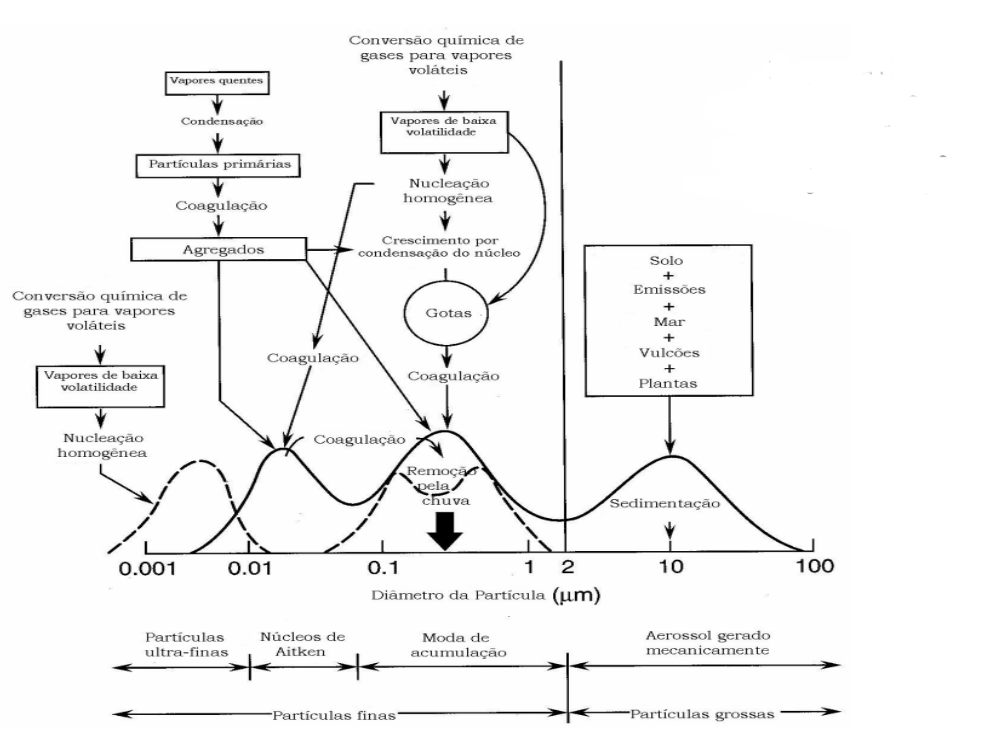
\includegraphics[width=0.8\textwidth]{../inputs/images/modas_aerossol.png}
  \caption{Esquema da distribuição de tamanho do aerossol atmosférico 
           \citep{finlayson1999} \label{fig:modas_aerossol}}
\end{center}
\end{figure}

O material particulado fino $MP_{2,5}$ engloba as partículas 
ultra-finas, a moda de nucleação e a moda de acumulação.  

O $MP_{2,5-10}$ tende a ficar retido na parte superior do sistema respiratório, 
enquanto que $MP_{2,5}$ tem maior facilidade para penetrar e atingir 
os alvéolos pulmonares e corrente sanguínea, 
podendo comprometer significativamente a saúde humana. 

O $MP$ pode ser emitido por diferentes fontes antropogênicas ou naturais e, 
também, pode ser gerado secundariamente na atmosfera, através de 
reações químicas, por exemplo. 

O $MP_{2,5}$ representa uma ameça a saúde humana, pois além 
do alto poder de penetração no sistema respiratório humano,
é gerado pelo processo de conversão gás-partícula, sendo esses 
gases muitas vezes tóxicos.

No $MP_{2,5}$ encontra-se principalmente íons $SO_4^=$, 
íons $ NO_3^-$, carbono elementar, carbono orgânico, 
elementos traços como metais 
(cádmio, níquel, vanádio, zinco, cromo, ferro, mercúrio), 
sulfatos e nitratos \citep{finlayson1999}. 

Compostos como nitrato e sulfato de amônio são poluentes secundários,
pois óxido de nitrogênio $NO_x$ e amônia $NH_3$ formam nitrato de amônio. 
Dióxido de enxofre $SO_2$ e amônia $NH_3$ formam o sulfato de amônio. 

Na moda grossa $MP_{2,5-10}$ há poluentes formados por processos mecânicos, 
como poeira de solo, fuligem, polens, metais alcalinos, entre outros. 
%%%%
\subsection{Black Carbon}

\textbf{Black Carbon} é um nome genérico que se da aos componentes
absorvedores de luz que compõe o material particulado e é formado pela combustão
incompleta de combustíveis fósseis, biocombustível e biomassa.
É encontrado predominantemente na fração fina do material particulado
e dependendo da região, representa mais da metade da massa do $MP_{2,5}$. 
Sua principal fonte em cidades são veículos automotores, 
especialmente os movidos a óleo combustível \citep{petzold2013}. 

Exposição a \textbf{Black Carbon} causa problemas respiratórios, 
cardiovasculares e morte prematura \citep{jacobson2014}.

BC particulate is one of the most harmful air pollutants
found in urban environments and is emitted by the incomplete
combustion of carbon-containing materials such as biomass
and fossil fuels. 

BC is made up of chains of spherules, has
diameters in the 10–50 nm range, has a non-zero imaginary
part of the refractive index, absorbs visible radiation, has a
vaporization temperature near 4000 K and is insoluble in
water and common organic solvents (Bond et al., 2013). In
the early 1980s the World Health Organization (WHO)
recognized the effects of BC particles on human health and
formulated the first guidelines for exposure limits to BC.
Because of its small size, BC particulate can reach the
lower respiratory tract, potentially carrying toxic chemical
species deposited onto their porous surface. Diesel fumes –
known for containing a high load of BC– have been
reclassified by the WHO from ‘probably carcinogenic’ to
‘carcinogenic’. Despite their short life span of 1 to 2 weeks
(in the absence of precipitation), BC absorbs incoming solar
radiation, and is the second most important man-made
agent of climate change, following carbon dioxide (Bond
et al., 2013)

In addition to BC particles emitted by industries, power
plants (ALA, 2011) and traffic, urban areas can be subject
to plumes of BC from local open burning and the outflow
of smoke from biomass fires (e.g., Saarikoski et al., 2007;
Targino et al., 2013).

Open burning involves the combustion
of any matter in open space and the emission of pollutants
(BC, organic carbon, inorganic species, polyclinic aromatic
hydrocarbons, dioxins, among others) directly into the
ambient air without passing through any duct filtration,
causing nuisance of smoke and odor.

The main burning activities that affect the urban air
quality are combustion of crop residue, land clearing debris
and house waste (Lemieux et al., 2004).

and frequently observed in rural areas and
neighborhoods with poor waste handling logistics or to
avoid paying for waste collection service.

Domestic waste
comprises a mix of organic (e.g., food and garden debris)
and non-organic waste (e.g., plasticized wrappings and
other polymeric materials) which burn with uncharacterized
emission factors. While governments are engaged to curb
industrial and traffic emissions in response to environmental
regulations, BC emissions from open burning dominate
global emission inventories, especially between 20°N and
30°S (EPA, 2012).

%%%%
%\subsection{Meio Ambiente}
%Ao depositar em folhas, as partículas impedem a absorção de luz. 
%Efeitos na visibilidade.
%Efeitos na formação de nuvens.


